\chapter{Materials and Methods}
\label{chap:materials-and-methods}

This chapter deals with background information relevant for your thesis, including physiological background, existing research on the topic, and mathematical and other preliminaries required to understand the novel concepts presented in the following chapter.
It is also often called \emph{Fundamentals} or \emph{Background}.

\section{Writing the background chapter}
As stated above, this chapter should contain the relevant background information that is required to follow the developments and discussions in the following (main) chapters.
Once you're beginning to write your thesis, you have probably learned a lot about your subject, and hence it will feel good to write down all that newly-gained knowledge in the background chapter.
It is therefore important to stress that you should \emph{not} use this chapter to write down all the background knowledge you have about the subject of your thesis.
This is \emph{not} intended to be a comprehensive textbook-style chapter that explains everything there is to know about the topic of the thesis.
Instead, really try to focus on \emph{just} the information which is necessary to understand the following chapters.
As a rule of thumb, the background chapter should generally not exceed 15 pages.

As an important corollary, it follows that \emph{writing the background chapter first is a bad idea}, because if you have not yet written the other chapters, how can you know which information you need to provide in the background chapter?
You should -- at the very least -- know the detailed structure for your \emph{whole} thesis precisely before beginning to write the background chapter.
Otherwise, you will probably find yourself rewriting or even removing large parts of this chapter later on.
For more details on the structure of the thesis writing process, refer to \cref{chap:concept}.

\section{\LaTeX's features}

This section provides a very brief introduction to writing a thesis with \LaTeX. 
It is important to know that \LaTeX\ is not a WYSIWYG (what you see is what you get) program like other text editors, such as Microsoft Word.
Instead, it much more resembles a programming language, in which you construct your text by proper usage of syntax.
The ``source code'' is your \LaTeX\ file (\texttt{.tex}). 

As in other programming languages, it is possible to insert comments in \LaTeX\ that are not visible in the final text, using the \% sign (refer to the source code for this paragraph in \texttt{materials\_and\_methods.tex} to see an example).
% This is not visible in the generated pdf, for example.
Line breaks are not of importance while writing the text, since they are created automatically during compilation.
Paragraph breaks are inserted automatically wherever there is a blank line in the source file.
The general formatting of the whole document can be customized precisely, but for the beginning, the default formatting provided in this template should be sufficient.

One of the big advantages of \LaTeX\ is its strong support for typesetting mathematical formulae, see \cref{sec:equations}.
The print quality achieved with \LaTeX\ formulae is hardly matched by any other program, let alone free of charge.
Also, references to your equations using the correct equation numbers can easily be used and maintained even while you change your document, insert new formulae that change the numbers of all equations, and so on.
Citing other works and providing a nicely compiled list of references is very easy in \LaTeX as well, see \cref{sec:citation}.

The following sections are not very useful if you just look at them in their compiled (pdf) form, but if you read the source code at the same time, it is easy to understand how different elements are constructed. 
You should try to compile the file yourself and compare the results. 
If there are any differences, check if your \LaTeX\ configuration is correct.

\section{Getting started with Latex}
\label{sec:getting-started-with}

To get started with Latex, you need...
\begin{enumerate}
\item A tool that generates a PDF file out of a bunch of *.tex and *.bib files.
On Windows, this is typically \swname{MikTex} (\url{http://miktex.org/download}).
\item A text editor. This can be as simple as \swname{Notepad++} (\url{https://notepad-plus-plus.org/}), but many would recommend an IDE that provides further convenience features. \swname{TexMaker} (\url{http://www.heise.de/download/texmaker.html}) and \swname{TexStudio} (\url{http://www.texstudio.org/}) are two well-known examples.
\end{enumerate}
If you have these two installed on your PC, you're ready to go!
There is a wealth of references and tutorials on the internet that deal with Latex.
What follows is a small list compiled based on my personal preferences.
\begin{itemize}
\item ShareLatex currently provides - to my taste - the best introduction and reference on a number of Latex-related topics: \url{https://www.sharelatex.com/learn}.
\item Latex-Wikibooks often prove useful if you're really looking for a reference of the available symbols, e.g. \url{https://en.wikibooks.org/wiki/LaTeX/Mathematics} or \url{https://en.wikibooks.org/wiki/LaTeX/Tables}.
\item There is a neat little online tool available which provides users with hints on available Latex commands based on the user's drawing of the desired symbol: \url{http://detexify.kirelabs.org/classify.html}.
\item Malte Schmitz from the Universität Lübeck also provides good introductory material in German: \url{http://www.mlte.de/layout}.
\end{itemize}


\section{Figures in Latex}
Figures should represent an essential component of your thesis, as they are excellent tools for effectively communicating information on complex issues to your reader.

\subsection{Creating good scientific figures}
While it is not easy to create visually appealing figures that represent information in the most accessible way, this is a skill that can be learned over time by reading various tutorials on the topic, carefully examining the works of other authors, and always reviewing one's own figures critically in this regard.
A good figure should be both functional by effectively conveying the relevant information, and visually appealing to the reader.
In \emph{very} few cases, a standard figure generated using, e.g., Matlab or python should be included directly in a scientific document without further modification and \glqq tuning\grqq.

To achieve functionality, the creator of a figure should think hard about the information which the figure should convey to the reader, and the best way to depict this visually. 
No unnecessary details should be present in the figure, because they will distract the reader from the main content -- grid lines, for example, are not really necessary in many plots and represent a distraction.
Every element of the figure that is not completely self-explanatory should be labeled.
The colors of elements should be selected in a meaningful way, i.e., very different elements should have clearly differing colors (blue and red, for example), while similar elements should have colors indicating that they belong together.
For example, if two different versions of an algorithm are compared to a third, very different algorithm, one might choose two similar (but still clearly distinguishable) colors for the first two, and a very different color for the third one.
See \url{www.colorbrewer2.org} for a list of color maps for many different use cases.
(There are packages available for many different programming languages, including python and Matlab, which implement the colorbrewer2 color maps.)

To make the figure visually appealing, care should be taken to make the figure neither too large (wasting space and making the figure look disproportionate in relation to its surroundings) nor too small (obscuring important details), and to pick a  color map that looks pleasing.
Screen shots and bitmap graphic files should generally be avoided, because they often look bad when scaled, have the wrong dimensions, etc.
Text size in figures should be a little bit smaller than normal text size, but still easily readable.
Finally, it is very important to ensure consistent formatting between figures in the thesis: ideally, they should all use the same color code, text style and size, and generally have the same \glqq look and feel\grqq.

A minimal checklist regarding the preparation of good scientific figures can be found in the \emph{Scientific Writing Checklist} that comes with this document.
A very brief introduction to clean and clear figure design can be found in, e.g., \url{https://youtu.be/UuL6wPGTJZQ}.
For more details on how to create good scientific figures, refer to, e.g., \textcite{Tufte1990, Ware2008, Few2012, Rougier2014}.
In the following, the rather technical aspect of how to generate and include figures in Latex will be considered, and several options will be discussed.

\subsection{Including figures in a Latex document}
\Cref{fig:sfap-schematic} shows a schematic of the geometry of of \gls{sfap} detection.
Note the extensive figure caption: many readers will first skim through your thesis and look at the figures, which should hence be as self-explanatory as possible.
\begin{figure}
  \centering
  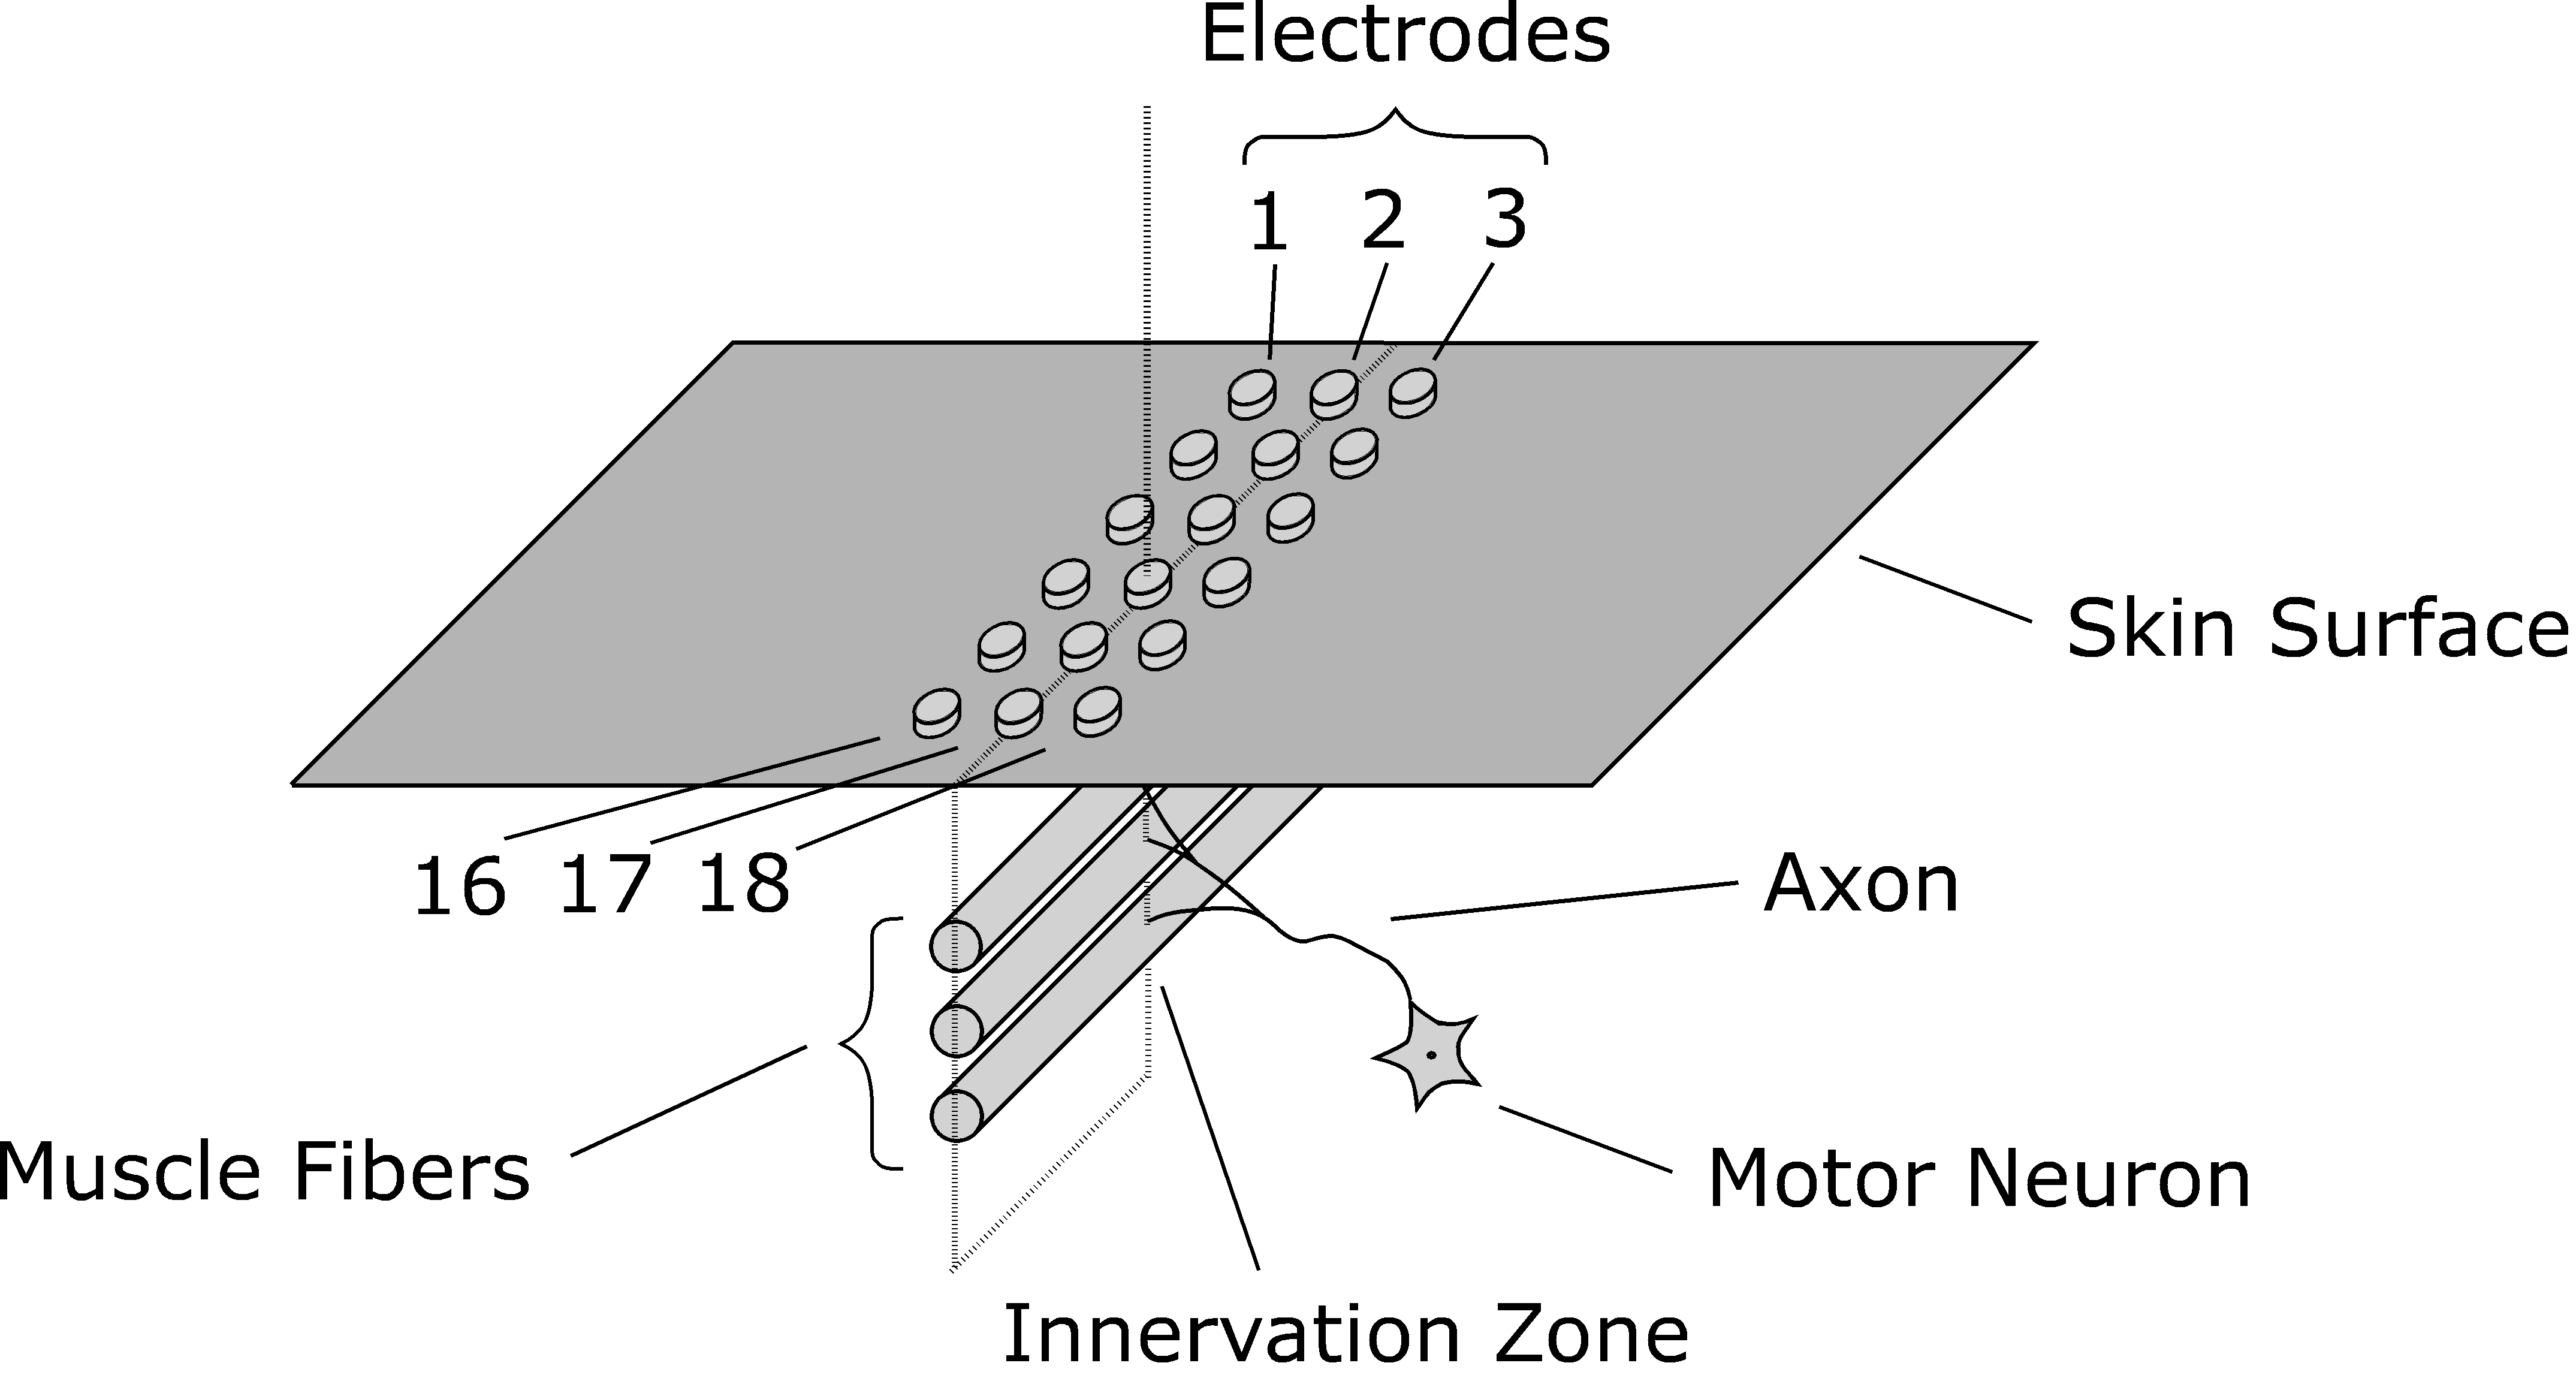
\includegraphics[width=12cm]{sfap-schematic}
  \caption[Geometry of Single Fiber Action Potential (SFAP) measurements]{Schematic of the geometry in \acrfull{sfap} measurements of human muscle fibers. Shown are three muscle fibers at different depths in the muscle tissue, and a regular grid of $18$ recording electrodes on the skin surface. This figure has been produced using the \texttt{Inkscape} software.}
  \label{fig:sfap-schematic}
\end{figure}

As opposed to \cref{fig:sfap-schematic}, which is included here as an external graphics file, \cref{fig:simple-schematic} shows a simple electrical schematic that is created completely in Latex, using the \swname{circuitikz} package.
\begin{figure}[htbp]
  \centering
  \begin{circuitikz} \draw
    (0,0) to [V=$U_0$] (0,3)
    to [R=$R_I$, i=$I_R$] (3,3)
    to [R=$R_L$] (3,0)
    to [C=$C_P$] (0,0)
    ;
  \end{circuitikz}
  \caption{A simple electrical circuit, drawn in Latex using the \swname{circuitikz} package. Note how the font type and size are exactly the same as in the normal text body.}
  \label{fig:simple-schematic}
\end{figure}
This package is based on the powerful \swname{tikz} package which allows for drawing any kind of figure directly in Latex.
This bears a number of advantages:
\begin{itemize}
\item The resulting figures are vector graphics, i.e., they are small (hence not resulting in a final thesis pdf size of several MBs) and generally look good.
\item Font style and size is consistent with the rest of the document. This is a major problem when importing figures from other software, e.g., \swname{Matlab}. (Also compare \cref{fig:sfap-schematic}.)
\item Each figure created this way is completely reproducible and configurable in every aspect.
\end{itemize}

Another package that is also based on the \swname{tikz} package is the \pgfplots{} package which enables the user to create plots either completely in Latex, or import data\footnote{For importing data in pgfplots, these are best exported to a \texttt{csv} file, e.g. using \texttt{csvwrite} in \matlab{} or \texttt{numpy.savetxt} or \texttt{pandas.DataFrame.to\_csv} in \python{}.} from an external program (e.g., \matlab{} or \python{}) and generate a nice-looking plot from this data using \swname{tikz} (with the advantages mentioned above).
\Cref{fig:matlab} shows an exemplary comparison of a plot exported directly from \matlab{} and the same data points exported to a data file and plotted using \pgfplots{}.
(It also shows how to create multiple subfigures inside a single figure.)
\begin{figure}[htbp]
	\centering
	% subfigure parameters are alignment (t=top) and subfigure width
	\begin{subfigure}[t]{.5\textwidth}
		\centering
		% figure width is set to the same width as during plot export in Matlab
		% to ensure correct font scaling
		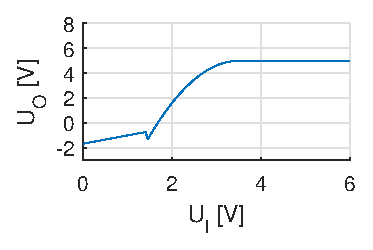
\includegraphics[width=2.5in]{figures/generated/ex2.eps}
		\caption{}
	\end{subfigure}%
	\begin{subfigure}[t]{.5\textwidth}
		\begin{tikzpicture}
			\pgfplotstableread[col sep=comma]{data/generated/data_analytical.csv}\dataana
		
			\begin{axis}[
	          axis x line=center,
	          axis y line=left,
	          xlabel=$U_{\text{in}} \, (\si{V})$,
	          ylabel=$U_{\text{out}} \, (\si{V})$,
	          xmin=0,
	          xmax=6.5,
	          ymin=-3,
	          ymax=7,
	          grid=major,
	          width=2.5in,
			]          
	          \addplot+ [no markers, style=solid, line width=1.5pt]
	          table {\dataana};
			\end{axis}
		\end{tikzpicture}
		\caption{}
	\end{subfigure}
	\caption[This is the short caption for the Matlab figure that appears in the list of figures]{The same data points, (a) plotted using \matlab{} and exported to an \texttt{.eps} figure file, and (b) exported to a \texttt{.csv} file from \matlab{} and plotted using \pgfplots{}.
	Note how the font type and size of all labels in figure (b) agree nicely with those in the rest of the document.}
	\label{fig:matlab}
\end{figure}
\Cref{fig:rosenfalck} shows an example of a plot that is generated completely in \pgfplots{}, without any aid from an external program.
\begin{figure}[htbp]
    \centering
    \newcommand*{\scalefactor}{0.5}
    \begin{tikzpicture}
      \newcommand*{\Aros}{96}
\newcommand*{\Bros}{-90}
\pgfplotsset{set layers}
\begin{axis}[
  small,
  width = \scalefactor\textwidth,
  axis y line = left,
  axis x line* = bottom,
  x unit = mm,
  y unit = mV/mm,
  xlabel = $z$,
  ylabel = $\psi$,
  xmin = -15,
  xmax = 2,
  ymin = -79,
  ymax = 39,
  xtick = {-10, -5, 0},
  ]

  \addplot [
  domain=-15:2, 
  samples=1000, 
  color=blue,
  ]
  {x>=0 ? 0 : -3*\Aros*x^2*e^x-\Aros*e^x*x^3}
  node[pos = 0.03,
       pin = 70 : {$\psi$}] {};

\end{axis}

\begin{axis}[
  small,
  width = \scalefactor\textwidth,
  axis y line = right,
  axis x line = none,
  x unit = mm,
  y unit = mV/mm^2,
  xlabel = $z$,
  ylabel = $\psi'$,
  xmin = -15,
  xmax = 2,
  ymin = -59,
  ymax = 119,
  ]

  \addplot [
  domain=-15:2, 
  samples=1000, 
  color=purple,
  ]
  {x<0 ? -(6*x+6*x^2+x^3)*\Aros*e^x : 0}
  node[pos = 0.02,
       pin = 70 : {$\psi'$}] {};
\end{axis}                      

    \end{tikzpicture}
  \caption[Plots of Rosenfalck's model function for the \acrlong{iap}]{Plots of the \acrfull{iap} model function proposed by \textcite{rosenfalck69}, generated using the \pgfplots{} package.
  Figure reproduced from \textcite{Petersen2015}.}
  \label{fig:rosenfalck}
\end{figure}

The \pgfplots{} package has one drawback, which is at the same time its greatest advantage: it generates \emph{vector graphics}.
Vector graphics have a number of significant advantages over raster graphics formats like \texttt{jpeg} and \texttt{png}.
However, when there is \emph{a lot} of data points in a figure, and hence a huge amount of vectors is required to accurately represent the figure, vector graphics tend to become very large and very inefficient to generate and view.
For such figures, raster graphics are usually preferrable -- however, one would still like to achieve things like consistent font size and type between the figure and the surrounding document.
One way to achieve this is by using the \gnuplot{} software package.
\gnuplot{} essentially provides a simple scripting language that can be used interactively or script-based to generate, view, and export figures from scratch or using existing data.
\Cref{fig:gnuplot-emg} shows a rather sophisticated figure containing EMG signals that has been generated using \gnuplot{}.
For more information, refer to the accompanying script file \texttt{scripts/emg-raw-plots.gp} that generated this figure, and to the \gnuplot{} homepage and various tutorials available on the web.
\begin{figure}[htbp]
	\centering
	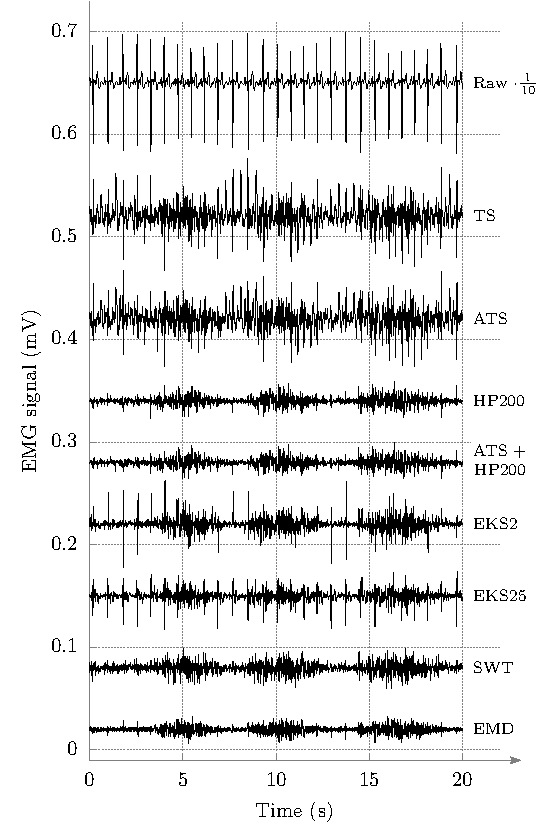
\includegraphics{figures/generated/emg-signals}
	\caption[This is the short caption for the EMG figure that appears in the list of figures]{Exemplary subset of the measurements taken from subject 7, raw (plotted with a scaling factor of $\frac{1}{10}$) and processed by the various ECG removal algorithms described in the text. All signals are zero-mean, with offsets added for illustrational purposes only.
	Due to the huge amount of data points, representing this figure in a vector graphics format (using, e.g., \pgfplots) would be very inefficient. 
	Here, the figure has been produced using the \gnuplot{} software in a raster graphics format, while still achieving nice and consistent visual formatting.}
	\label{fig:gnuplot-emg}
\end{figure}

\section{Referencing}
\label{sec:citation}
Every statement that you make in your thesis should either be supported by evidence (theoretical or empirical) provided in your thesis, or by citation of an appropriate literature reference.
In the present chapter (materials and methods) in particular, you should provide a lot of references, e.g., to scientific articles~\cite{farina99}, books~\cite{plonsey07}, book chapters~\cite{rodriguez-falces12}, PhD theses~\cite{fevotte03}, or software projects~\cite{r-project} that you used during the creation of your thesis.
You must provide a reference whenever you make a statement that is not a result of your own (experimental or theoretical) work, but rather taken from a literary source.
When selecting sources to cite, preference should be given to high-quality sources published in respected scientific journals (or books), wherever possible.
Moreover, one should always try to cite the original source where a subject was discussed first or an algorithm was proposed first, instead of secondary sources.
For example, regarding the infamous Kalman filter, one should always cite the original paper published by \textcite{Kalman1960} instead of the many papers published later on (variations of) the same subject.

Sometimes, you should explicitly name authors, such as \textcite{farina99}, who wrote a seminal article on the mathematical modelling of \gls{emg} measurements (see the Latex source document to see how this textual reference is created automatically)\footnote{Note how the \gls{emg} acronym is clickable and leads to the definition of this acronym in the glossary.
This is one of the many features of the \swname{glossaries} package.}.
In some cases -- especially when describing the fundamentals of your research -- you will have entire paragraphs that are based on a single, significant reference on the subject you describe.
In this case, it is neither necessary nor useful to cite said reference after each phrase.
One acceptable solution is to have a phrase in the beginning of the paragraph or section that acknowledges the source and states clearly that the entire following paragraph is based on this source.

Figures may be reproduced from sources, in which case the source must of course be acknowledged accordingly -- refer to \cref{fig:rosenfalck} for an example of how this can be done.
It is also considered good scientific practice to provide citations for the software packages that you have used, considering that these are often the result of many years of scientific work~\cite{r-project, Wickham2009}.
Many software packages provide information on how to cite them on their project web pages.

Finally, a bibliography can be created automatically, based on the order in which you have cited sources (see the appendix for an example).
This can be achieved using various tools and packages, which all require a separate file (often called \texttt{references.bib}) containing bibliographic information on the cited sources.
In this template, the \texttt{biblatex} package in combination with the \texttt{biber} software is used.
Usage is simple: After compiling your document once with \texttt{pdflatex}, a file \texttt{main.bcf} is generated, which essentially contains a list of the cited sources.
Next, running \texttt{biber main} on the command line combines this generated list with the \texttt{.bib} file and generates a new file \texttt{main.bcf} that contains the required bibliographic information, using the correct order and citation style.
Afterwards, run \texttt{pdflatex} again, to incorporate this bibliographic information in the generated document.
This process has to be repeated every time a new source is cited in the main document, and each time bibliographic information in the \texttt{bib} file is added or changed.
Note that there are various software packages available that enable easy handling of bibliographic data and automatic generation of a corresponding \texttt{bib} file, e.g. the open source package \texttt{JabRef}.

\subsection{This is a subsection}
See the source code for how this is achieved.

\subsubsection{This is a subsubsection}
Note that the different appearance of chapters, sections, subsection and subsubsections can be customized if desired.

\section{Equations}
\label{sec:equations}
If you are going to write more than a few equations in your thesis, it is highly recommendable to use macros to define each variable that occurs.
This way, if you decide to rename the velocity from $v$ to $v_0$ (see the source code of this section for how to include mathematical symbols like $v$ in normal text) everywhere in your thesis later on during the process of writing, you will only have to change the definition of the macro used for this variable.
For example, in
\begin{equation}
  \label{eq:1}
  \vel = \frac{\diff \loc}{\diff t}
\end{equation}
and
\begin{align}
  \label{eq:2}
  \acc &= \frac{\diff \vel}{\diff t} \nonumber \\
  &= \frac{\force}{\mass},
\end{align}
each of the variables is defined using a macro.
Always keep in mind that formulae should be treated as a normal part of a sentence and thus can and have to contain punctuation marks!
\emph{Never} should any sentence start with a mathematical symbol.
Finally, here comes an example of how to reference equations \eqref{eq:1} to \eqref{eq:2}.
These references will update automatically if you decide to move these equations to a different part of the thesis, or if another equation is inserted between these two, hence changing equation numbering.

\section{Pseudo code}
Algorithm \ref{alg:euclid} is an example of how pseudo code can be represented in Latex.
Of course there are, as with anything in Latex, many options available to achieve this goal.
Here, the \swname{algpseudocode} package is employed.
\begin{algorithm}
  % Example code due to
  % http://tex.stackexchange.com/a/230789/64293
    \caption{Euclid's algorithm}
    \label{alg:euclid}
    \begin{algorithmic}[1] % The number tells where the line numbering should start
        \Procedure{Euclid}{$a,b$} \Comment{The g.c.d. of a and b}
            \State $r\gets a \bmod b$
            \While{$r\not=0$} \Comment{We have the answer if r is 0}
                \State $a \gets b$
                \State $b \gets r$
                \State $r \gets a \bmod b$
            \EndWhile\label{euclidendwhile}
            \State \textbf{return} $b$\Comment{The gcd is b}
        \EndProcedure
    \end{algorithmic}
\end{algorithm}




%%%%% Emacs-related stuff
%%% Local Variables: 
%%% mode: latex
%%% TeX-master: "../../main"
%%% End: 
